%(BEGIN_QUESTION)
% Copyright 2009, Tony R. Kuphaldt, released under the Creative Commons Attribution License (v 1.0)
% This means you may do almost anything with this work of mine, so long as you give me proper credit

The {\it activated sludge} process is used in municipal wastewater treatment to decompose organic matter suspended in the water.  A sizeable culture of naturally-occurring bacteria (the same strains at work in your own gut) eat the organic matter in the wastewater as the water passes through the aeration chamber.  These bacteria are oxygen-consuming (``aerobic''), and so must be given plenty of oxygen to respirate.  An air blower provides this air so the bacteria may thrive in the aeration chamber:

$$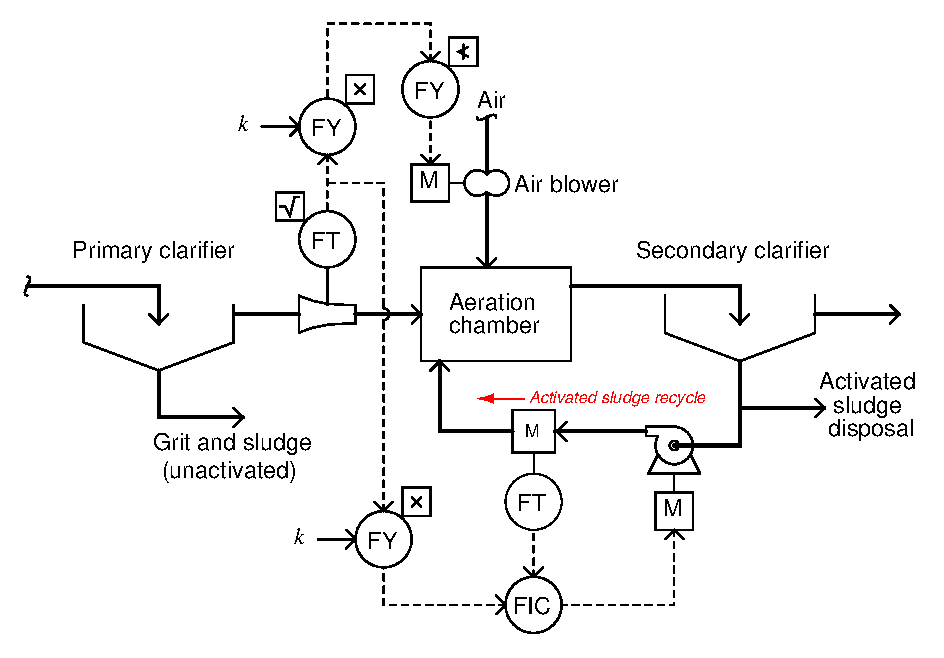
\includegraphics[width=15.5cm]{i04067x01.eps}$$

Suppose the magnetic flowmeter used to measure sludge recycle flow imparts a magnetic flux density of 0.2 Tesla across a flowtube 4 inches in diameter (10.16 centimeters, or 0.1016 meters).  Calculate the amount of voltage this flowtube will generate at a sludge flow rate of 0.67 cubic meters per minute.  Also, convert this sludge flow rate into units of gallons per minute.

\vskip 20pt \vbox{\hrule \hbox{\strut \vrule{} {\bf Suggestions for Socratic discussion} \vrule} \hrule}

\begin{itemize}
\item{} Explain why a magnetic flowmeter is ideally suited for this application, where the sludge has the approximate consistency (and appearance!) of peanut butter.
\item{} Will a magnetic flowmeter still work well if there is a substantial amount of non-conductive matter in the flowstream (e.g. rocks or air bubbles)?  Explain why or why not.
\item{} Identify any other flowmeter types you've learned about so far which may work well in this application as an alternative to the magnetic flowmeter.
\item{} Identify any other flowmeter types you've learned about so far which would {\it not} work well in this application as an alternative to the magnetic flowmeter, and explain why.
\item{} Identify the flowmeter type used to measure influent flow, and also explain why it has a square-root symbol next to it.
\item{} Explain what a {\it clarifier} vessel does, and the purposes each one serves in this process.
\item{} Demonstrate how to {\it estimate} numerical answers for this problem without using a calculator.
\end{itemize}

\underbar{file i04067}
%(END_QUESTION)





%(BEGIN_ANSWER)

\noindent
{\bf Partial answer:}

\vskip 10pt

Voltage = 27.99 millivolts

%(END_ANSWER)





%(BEGIN_NOTES)

$$E = Blv = {B d Q \over A} = {4 B Q \over \pi d}$$

\noindent
Where,

$E$ = Motional EMF (volts)

$B$ = Magnetic flux density (Tesla)

$l$ = Length of conductor passing through the magnetic field (meters)

$v$ = Velocity of conductor (meters per second)

$d$ = Diameter of pipe (meters)

$A$ = Cross-sectional flowing area of pipe (square meters)

$Q$ = Flow rate (cubic meters per second)

$k$ = Constant of proportionality

\vskip 10pt

0.67 cubic meters per minute is equal to 0.112 cubic meters per second.  A circular diameter of 4 inches equates to a cross-sectional area of 0.00810732 square meters.

\vskip 10pt

$$E = {(0.2) (0.1016) (0.112) \over 0.008107} = 27.99 \hbox{ mV}$$

\vskip 10pt

For those who intend to use the $E = Blv$ formula, velocity $v$ ends up being 1.377 meters per second.

\vskip 10pt

Converting the volumetric flow rate of 0.67 cubic meters per minute into gallons per minute:

$$\left({0.67 \hbox{ m}^3 \over \hbox{min}}\right) \left(100 \hbox{ cm} \over 1 \hbox{ m} \right)^3 \left(1 \hbox{ in} \over 2.54 \hbox{ cm}\right)^3 \left(1 \hbox{ gallon} \over 231 \hbox{ in}^3 \right) = 176.995 \hbox{ GPM}$$









\vskip 20pt \vbox{\hrule \hbox{\strut \vrule{} {\bf Virtual Troubleshooting} \vrule} \hrule}

This question is a good candidate for a ``Virtual Troubleshooting'' exercise.  Presenting the diagram to students, you first imagine in your own mind a particular fault in the system.  Then, you present one or more symptoms of that fault (something noticeable by an operator or other user of the system).  Students then propose various diagnostic tests to perform on this system to identify the nature and location of the fault, as though they were technicians trying to troubleshoot the problem.  Your job is to tell them what the result(s) would be for each of the proposed diagnostic tests, documenting those results where all the students can see.

During and after the exercise, it is good to ask students follow-up questions such as:

\begin{itemize}
\item{} What does the result of the last diagnostic test tell you about the fault?
\item{} Suppose the results of the last diagnostic test were different.  What then would that result tell you about the fault?
\item{} Is the last diagnostic test the best one we could do?
\item{} What would be the ideal order of tests, to diagnose the problem in as few steps as possible?
\end{itemize}














\vfil \eject

\noindent
{\bf Prep Quiz:}

The {\it activated sludge} process is used in industry to:

\begin{itemize}
\item{} Convert isopropyl alcohol into acetone (solvent)
\vskip 5pt 
\item{} Manufacture fast-setting concrete mixes
\vskip 5pt 
\item{} Refine heavy crude oil fractions into gasoline
\vskip 5pt 
\item{} Efficiently extract minerals from feedwater
\vskip 5pt 
\item{} Decompose organic matter suspended in water
\vskip 5pt 
\item{} Induce vomiting in victims of poisoning
\end{itemize}

%INDEX% Measurement, flow: magnetic
%INDEX% Process: activated sludge wastewater treatment

%(END_NOTES)


